\chapter{Diffusion Maps}
\section{Introduction}

Diffusion Maps are a technique for discovering underlying geometricity of a graph $G=(V,E)$ solely from the connectivity. We will put the technique to use in order to invert the GIRG generative process - go from a graph produced by a $d$-dimensional GIRG, and infer the original locations $(x_u)_{u\in V}$ of the vertices $x_u \in \T^d$.

The idea of Diffusion Maps is to analyse the diffusion process of random walking on the edges of the graph, and to characterise the probability cloud starting from one node in the graph as a sum of decreasingly important contributions, along the line of eigenvectors of decreasing eigenvalues from a diagonalisable matrix. The top $d$ contributions can then be used as a coordinate system to describe each point in the graph. By taking a large timestep diffusion cloud, the general relative location of the initial point is the main signal. The hope is that if connections (probabilistically) follow a geometry of $d$-dimensions, then the diffusion map coordinate system will capture / align with this real geometry.

The diffusion process is defined by the random walk 
\begin{equation}
  M_{ij} := P(X(t+1) = j | X(t)=i) = \frac{w_{ij}}{\deg(i)}
\end{equation}

\begin{align*}
  & M = D^{-1}W \quad & \text{transition matrix}\\
  & D_{uu} = \sum_{v\in V} W_{uv} \quad & \text{diagonal degree matrix}\\
  & W_{uv} = \begin{cases}1 & u \sim v \\0 & u \nsim v \end{cases} \quad & \text{adjacency matrix}
  \\
  & S = D^{-1/2} W D^{-1/2} \quad & \text{symmetric matrix}\\
  & \;\; = V \Lambda V^T \quad & \text{diagonalisation into orthonormal e-vectors}\\
  & \Phi = D^{-1/2} V = [\vec{\phi}_1, \vec{\phi_2}, ..., \vec{\phi_n}] \quad & \Psi = D^{1/2} V = [\vec{\psi_1}, \vec{\psi_2}, ..., \vec{\psi_n}]\\
  & \Phi^T \Psi = \Psi^T \Phi = I_{n \times n} \quad & \text{due to orthonormality of $V$}
\end{align*}
%
We use the diagonalisation of $S$ to write $M$ as 
\begin{align*}
  & M = D^{-1/2} S D^{1/2} = \Phi \Lambda \Psi^T \quad & \text{diffusion map representation}\\
  & \;\;\; = \sum_{k=1}^n \lambda_k \vec{\phi}_k \vec{\psi}_k^T &
\end{align*}
%
The biorthonormality $\langle \vec{\phi}_i, \vec{\psi}_j \rangle = \delta_{ij}$ means that $M \vec{\phi}_i = \lambda_i \vec{\phi}_i$ and $M^T \vec{\psi}_i = \lambda_i \vec{\psi}_i$. For a diffusion map representation of nodes, we order eigenvalues $\lambda_1 \geq \lambda_2 \geq ...$.
Notably the transition matrix satisfies $M\vec{1} = \vec{1}$ since $\sum_j \frac{w_{ij}}{\deg(i)} = 1$, which can be shown to be the largest eigenvalue $\lambda_1=1$; if the graph is connected then also $\lambda_2 < 1$. In particular then $\vec{\phi}_1 = c \vec{1}$.

Then the diffusion map representation of a node is then
\begin{align*}
  & e_i^T M = \sum_{k=1}^n \phi_i(k) \lambda_k^t \vec{\psi}_k \quad & \text{diff map of node $i$ after $t$ steps}\\
  & i \mapsto (\phi_2(i) \lambda_2^t,... \phi_{m+1}(i) \lambda_{m+1}^t) \quad & \text{m-truncated diff map representation}
\end{align*}
%
The truncated diffusion map summarises the distinguishing features of a node's random walk cloud after $t$ steps, by taking the scale factor of $\vec{\psi}_k$ ($\vec{\psi}_k$ itself is ignored as it's relatively normalisesd: $\vec{\psi}_k = \vec{d}^{1/2} \odot \vec{v}_k$ (TODO is this really normalised?)). Since $\vec{\phi}_1 = c \vec{1}$, the first coordinate is dropped as it's useless for distinguishing nodes. This corresponds to the fact that the diffusion cloud starting at any node converges as $t \to \infty$ to the same stationary distribution $\vec{\pi}_i = \frac{d_i}{\sum_j d_j}$.


We attempt to improve the diffusion map process for GIRGs. In particular, we'd like the random walk to prioritise edges going to nodes with low degree, as these are more likely to be the neighbours of the node in the underlying geometry. We do this by modifying the transition matrix $M$ to $\tilde{M}$ as follows:

\begin{align*}
  \tilde{M} = \tilde{D} M D^{-\gamma}
\end{align*}
Where $\tilde{D}$ is to normalise $\tilde{M}$ to ensure that it's still a row stochastic matrix: $\sum_j \tilde{M}_{ij} = 1$. The tuning parameter $\gamma > 0$ directly controls the bias towards low degree nodes: $M_{ij} d^{-\gamma}_j$ means that nodes $j$ with high $d_j$ have a relatively lowered transition probability.
This unfortunately messes up all our nice equations. $\tilde{M}$ is still row stochastic, which means it still has a largest magnitude eigenvalue $\lambda_1 = 1$, and by the Gershgorin circle theorem, all other $|\lambda_i| \leq 1$.

We can write it as $\tilde{M} = D_1 \Phi \Lambda \Psi^T D^{-\gamma}$. This does at least allow the decomposition $\tilde{M} = \sum_k \lambda_k \vec{\tilde{\phi}}_k \vec{\tilde{\psi}}_k$, where $\vec{\tilde{\phi}}_k = D_1 \vec{\phi}_k$ and $\vec{\tilde{\psi}}_k = D^{-\gamma} \vec{\psi}_k$. In particular, $\tilde{M} (D_2^{-1} \vec{\phi}_k) = \lambda_k D_1 \vec{\phi}_k$. This does not mean that $\tilde{M}$ has eigenvalues $\lambda_i$, rather they're slightly different.

Instead we hope that $\tilde{M}$ is diagonalisable as $\tilde{M} = BAB^{-1}$ for diagonal $A$, and use the corresponding diffusion map representation $i \mapsto (\vec{b}_2(i) a_2^t,... \vec{b}_{m+1}(i) a_{m+1}^t)$.

Actually no hope for diagonalisability is needed. This process can be viewed as modifying the adjacency matrix $W_{ij}$ to have not all $1$ weights, instead having weights e.g. $d_i^{-\gamma}d_j^{-\gamma}$. This is done all at the start, so then $S = D^{-1/2} W D^{-1/2}$ is well defined using $D_ii = \sum_{j \neq i} W_{ij}$, and $M = D^{-1} W$ is still a valid probability transition matrix. Indeed it involves $M_{ij} = \frac{W_{ij}}{D_{ii}}$ which comes out with the same $d_j^{-\gamma}$ weighting as previously hoped for.

Another interpretation of this is following:
heat kernel?? wtf. See Belkin Nyiogi Laplacian Eigenmaps for Dimensionality Reduction and Data Representation

The logic roughly goes: Belkin Nyiogi suggest converting a geometric distribution into a graph via $W_{ij} = e^{-||x_i - x_j||^2}{T}$ for some parameter $T > 0$. We're given a straight graph, but using the GIRG assumption, we know that $u \sim v$ means roughly that $r_{uv} \approxeq \left ( \frac{w_u w_v}{n} \right )^{1/d}$. I.e. we can plug this guess in to give smaller weights to edges between nodes with high degree, analgously to the above approach of setting $W_{ij} = d_i^{-\gamma} d_j^{-\gamma}$.

The way we benchmark all these approaches is by generating a graph $G$ with a GIRG (potentially a slightly wonky one), and looking at the correlation coefficient of pts and pts dm. We see that both heat kernel method and $D^{-\gamma}$ method outperform baseline, and $D^{-\gamma}$ method outperforms heat kernel method, using about $\gamma=0.9$. welp.
% % 
% The m-truncated diffusion map representation becomes the new r epresentation of nodes in the graph. The diffusion map is then a function $\R^n \to \R^m$. The first coordinate $\lambda_1$ is always $1$, corresponding to the stationary distribution of the random walk which all node diffusion maps converge to. This is useless for differentiating nodes and is hence dropped.

% Notably the transition matrix satisfies $M1 = 1$ since $\sum_j \frac{w_{ij}}{\deg(i)} = 1$, and it can be shown that it has eigenvalues $\lambda_1=1 \geq \lambda_2 \geq \lambda_3 \geq ...$.  





% Oh no $\vec{x}$.

% by the transition matrix $M = D^{-1}W$, where $D$ is the diagonal matrix with $D_{uu} = \sum_{v\in V} W_{uv}$ is the diagonal degree matrix, and $W_{uv}$ is the adjacency matrix, $W_{uv} = \begin{cases}1 & u \sim v \\0 & u \nsim v \end{cases}$. The matrix $S = D^{-1/2} W D^{-1/2}$ is a symmetrised version and hence is diagonalisable as $S = V \Lambda V^T$. Then the map $M = D^{-1/2} S D^{1/2} = D^{-1/2} V \Lambda (D^{1/2} V)^T = \Phi \Lambda \Psi^T$.

% In particular, starting at node $i$ (numbered $i=1,...,n$), the $t$th step diffusion cloud is $i \mapsto M^t_{ij} = (\Phi \Lambda^t \Psi^T)_{ij} = \sum_{k=1}^n \Phi_{ik} \lambda_k^t \Psi_{jk}$.

% So writing $\Phi = [\phi_1, \phi_2, ..., \phi_n]$ and $\Psi = [\psi_1, \psi_2, ..., \psi_n]$, we have that the $t$th step diffusion cloud is $i \mapsto \sum_{k=1}^n \phi_k(i) \lambda_k^t \vec{\psi}_k$. I.e. the diffusion map coordinate system is $\text{diffmap}_t(i) = (\lambda_2^t \phi_2(i), \lambda_3^t \phi_3(i), ..., \lambda_{d+1}^t \phi_{d+1}(i))$. The first coordinate is always $1$, it's the stationary distribution that all diffusion clouds converge to, so is discarded.

\section{Diffusion Maps on GIRGs}
If we have a graph $G$ which we know is generated from a $d$-dimensional GIRG, we can simply extract the $d$-truncated diffusion map coordinates of each node as an estimate for the original geometric location of the node.

If $d$ is unknown, diffusion maps present one way to infer the dimensionality by analysing the ordered sequence of eigenvalues $\lambda_2 < \lambda_3 < ...$. In theory there is a good cutoff point whereby the first $d$ eigenvalues are of similar large size, and the rest are much smaller. This indeed works well for graphs synthetically generated from GIRGs, not so well on real world graphs.


We see in \cref{fig:cube_diffmap_plots_d2} that the inferred first two diffusion map coordinates do fit a square quite well. In general the points will be centered around the origin, as all $\lambda_2, \lambda_3, ...$ eigenvalue eigenvectors will be orthogonal to the stationary distribution $\vec{\phi}_1 = k \vec{1}$ : they represent a deviation from the stationary distribution - e.g. for a node on the 1D line towards left end, it will need to put more diffusion probability on the left side nodes, and less on the right side nodes than the stationary distribution. The y-axis scale is small as $\lambda_2 < 1$, and is decreasing with $t$.

\subsection{Rescaling/Shifting Diffusion Maps}
The 0 centering can easily be fixed to be more Cube GIRG like by shifting the points $(\vec{x}_u)_i \gets (\vec{x}_u)_i + \min_v (\vec{x}_v)_i$.
If we are certain that the points should be distributed within the unit cube, then we can simply rescale separately along each dimension: $x \gets \frac{x - x_{\min}}{x_{\max} - x_{\min}}$.
If furthermore we're certain that the distribution within the unit cube should be relatively uniform, we can perform a coordinatewise "uniformify" procedure that replaces $(x_u)_i$ with its percentile value compared with other $(x_v)_i$. \cref{fig:diffmap_uniformed_vs_nonuniformed} shows the "uniformify" procedure in action. Notably on real graphs where the truncated diff map coordinates are not guaranteed to be independently distributed, coordinatewise percentile mapping can lead to slightly odd results - see socfb-Amherst where there's a strong $x_1 = 1 - x_2$ correlation for small $x_1$. It's still a good improvement over the original non rescaled diffusion map.

% The decreasing diffusion map scaling can be see either as a bug or a feature. If we are certain that the points should be distributed within the unit cube, then we can simply rescale separately along each dimension: $x \gets \frac{x - x_{\min}}{x_{\max} - x_{\min}}$. If furthermore we're certain that the distribution within the unit cube should be relatively uniform, we can perform a coordinatewise "uniformify" procedure that replaces $(x_u)_i$ with its percentile value compared with other $(x_v)_i$. \cref{fig:diffmap_uniformed_vs_nonuniformed} shows the "uniformify" procedure in action. Notably on real graphs where the truncated diff map coordinates are not guaranteed to be independently distributed, coordinatewise percentile mapping can lead to slightly odd results - see socfb-Amherst where there's a strong $x_1 = 1 - x_2$ correlation for small $x_1$. It's still a good improvement over the original non rescaled diffusion map. 

Critically since there is no guarantee that the scaling of diffusion map coordinates is the same as the original GIRG coordinates, using some kind of prior knowledge to rescale the diffusion map is important to yield geometric information with meaningful inter-point distances.

\paragraph{Rotated Points} One issue with diffusion maps as seen in \cref{fig:cube_diffmap_plots_d2}, the 2D GIRG's 2D-truncated diff map looks like a rotated square. While the diffusion map has successfully extracted geometric information from the graph, it's not done so in the original basis. This phenomenon can make rescaling and uniformifying to the unit cube a little questionable.

\paragraph{Non-cube GIRGs} However in practice, real graphs never have an equal balance in geometric dimension importance. This is easiest to understand with the example of a weighted euclidean norm setup, where it could be that a 2D GIRG's true 1st geometric dimension (between $[0, 1]$) is much more important than its 2nd geometric dimension in influencing edge probabilities: $\norm{x - y} = \sqrt{a (x_1 - y_1)^2 + b(x_2 - y_2)^2}$.
The diffusion map is solving an eigenvalue problem that is like a maximsation of diffusion explainability. If $a > b$, then by maximisation the first diffusion map coordinate $\varphi_1(u)$ is likely to be very similar to $(\vec{x}_u)_1$. Only if $a=b$ is there no preference between $(\vec{x}_u)_1$ and $(\vec{x}_u)_2$, making a rotation possible.
Hence the points $(\varphi_1(u), \varphi_2(u))_{u \in V}$ are likely to end up as a rectangle, not a rotated square; the variation in first coordinate will be greater than in the second.

In this light the relative $\lambda_2 > \lambda_3 > ...$ scaling can be seen as a feature not a bug, if the hypothesis space of generative graph models is to be expanded to cuboid (non-cube) GIRGs.
The relative flatness of $\lambda_2, \lambda_3, \lambda_4, \lambda_5$ line segment in \cref{fig:cube_diffmaps_d4} is a testament to the underlying cube GIRG that generated the graph.




% In this case, the diffusion map coordinates will have a larger scale for the $\lambda_2$ coordinate than the $\lambda_3$ coordinate, and the points will look like an elongated rectangle.

% the distance: $\norm{x - y} = \sqrt{a (x_1 - y_1)^2 + b(x_2 - y_2)^2}$. In this case, the diffusion map coordinates will have a larger scale for the $\lambda_2$ coordinate than the $\lambda_3$ coordinate, and the points will look like an elongated rectangle. The flatness of $\lambda_2, \lambda_3, \lambda_4, \lambda_5$ line segment in \cref{fig:cube_diffmaps_d4} is a testament to the cube (and non cuboidness) of the underlying GIRG that generated the graph.


% (relatively uniformly) distributed within the unit cube, then we can simply rescale separately along each dimension.
% A linear coordinatewise scaling $x \gets \frac{x - x_{\min}}{x_{\max} - x_{\min}}$ works, or more extremely a coordinatewise "uniformify" procedure that replaces $(x_u)_i$ with its percentile value compared with other $(x_v)_i$.
% In \cref{fig:diffmap_uniformed_vs_nonuniformed} we see uniformified versions of a generated 2D GIRG, and the socfb-Amherst41 graph.

% Seen as a feature, the relatively different scaling allows as a natural correction to the potential non equivalence of different dimensions. For instance in a weighted euclidean norm setup, it could be that a 2D GIRG's true 1st geometric dimension (between $[0, 1]$) is much more important than its 2nd geometric dimension in determining the distance: $\norm{x - y} = \sqrt{a (x_1 - y_1)^2 + b(x_2 - y_2)^2}$. In this case, the diffusion map coordinates will have a larger scale for the $\lambda_2$ coordinate than the $\lambda_3$ coordinate, and the points will look like an elongated rectangle. The flatness of $\lambda_2, \lambda_3, \lambda_4, \lambda_5$ line segment in \cref{fig:cube_diffmaps_d4} is a testament to the cube (and non cuboidness) of the underlying GIRG that generated the graph. 


% TODO put in some eigenvalue plots

\begin{figure}
    \centering

    \begin{subfigure}{0.49\textwidth}
      \centering
      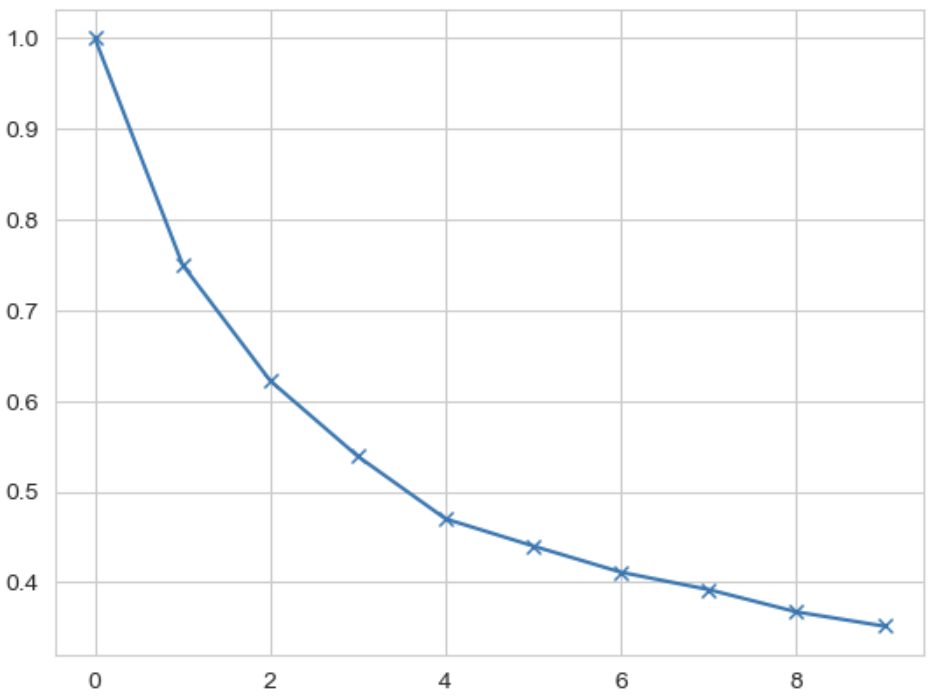
\includegraphics[width=\linewidth]{figures/diffmap_1d.png}
      \caption{$d=1$}
    \end{subfigure}
    \hfill
    \begin{subfigure}{0.49\textwidth}
      \centering
      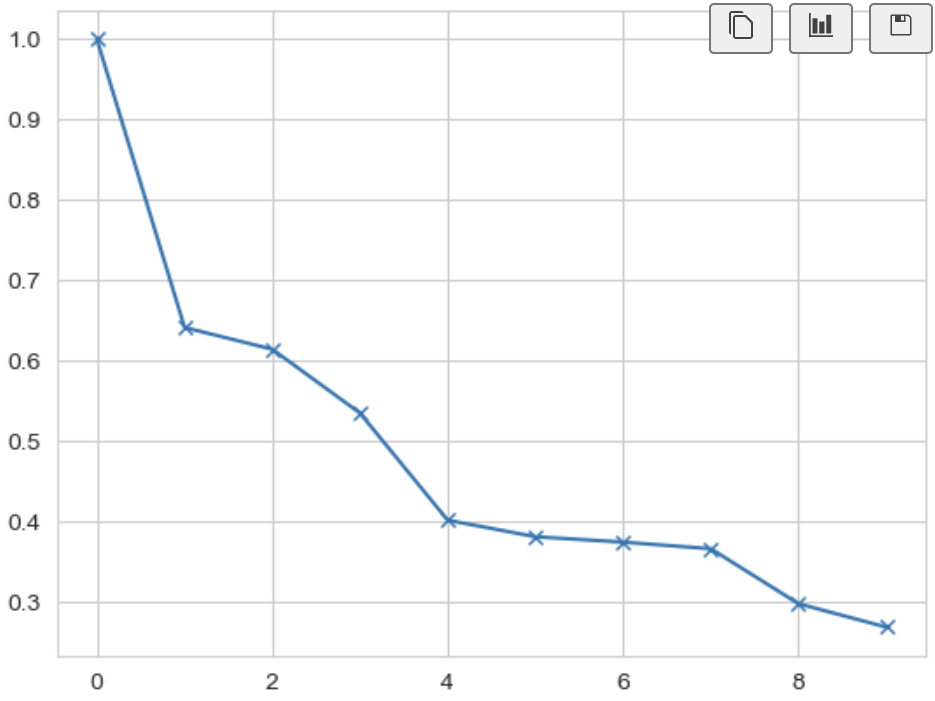
\includegraphics[width=\linewidth]{figures/diffmap_2d.png}
      \caption{$d=2$}
    \end{subfigure}
  
    \vspace{1em}
  
    \begin{subfigure}{0.49\textwidth}
      \centering
      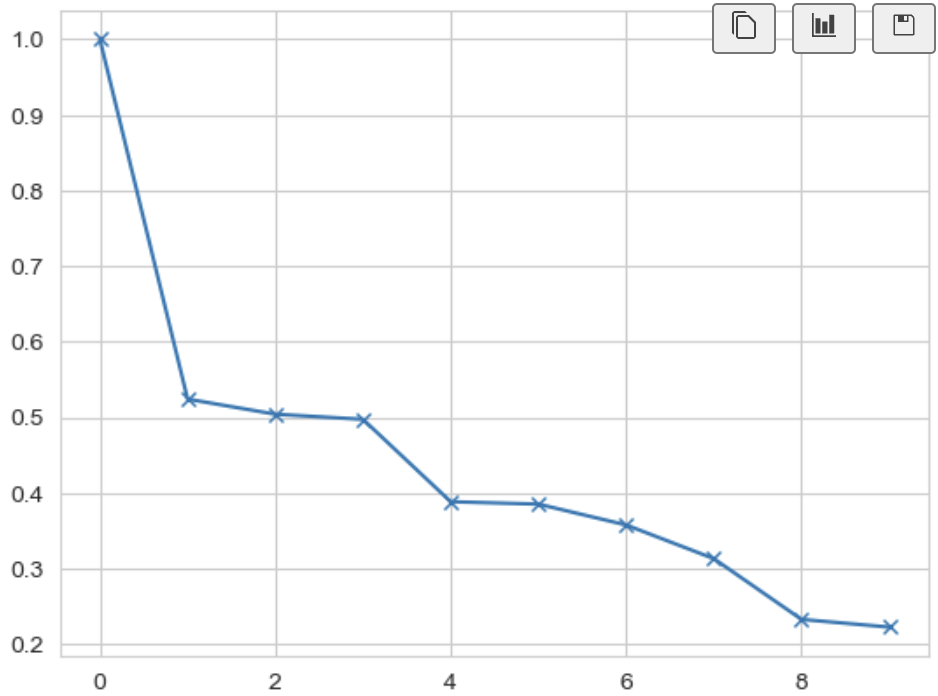
\includegraphics[width=\linewidth]{figures/diffmap_3d.png}
      \caption{$d=3$}
    \end{subfigure}
    \hfill
    \begin{subfigure}{0.49\textwidth}
      \centering
      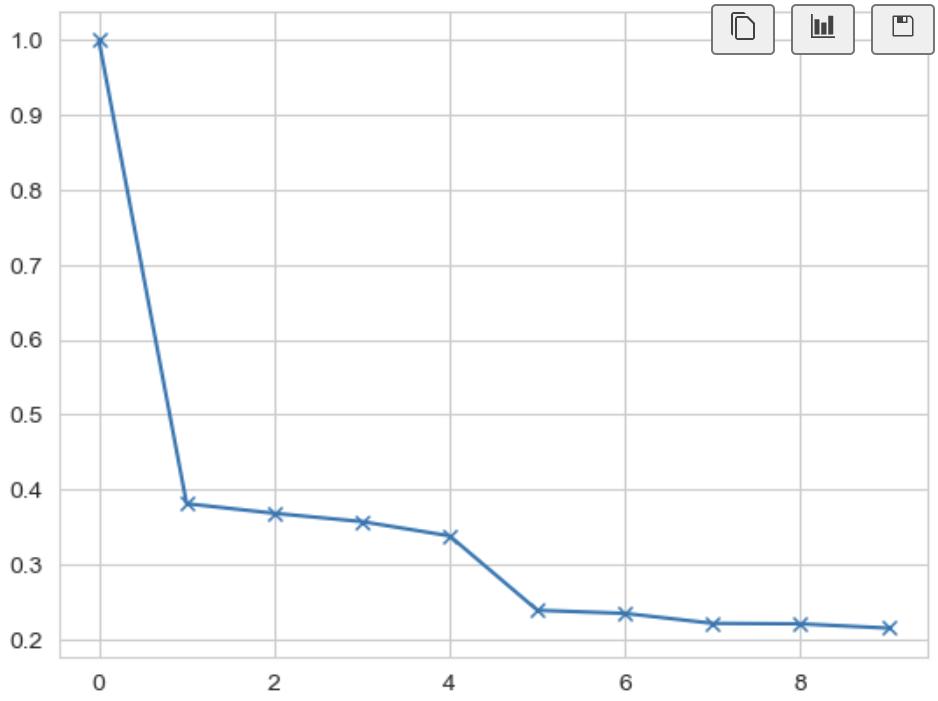
\includegraphics[width=\linewidth]{figures/diffmap_4d.png}
      \caption{$d=4$}
      \label{fig:cube_diffmaps_d4}
    \end{subfigure}
  
    \caption{Diffusion map eigenvalues (including $\lambda_1 = 1$) for a $n=2000, \tau=2.5, \alpha=1.3$ Cube GIRG with $d=1,2,3,4$ dimensions.}
    \label{fig:cube_diffmaps_d1to4}
\end{figure}

\begin{figure}
    \centering

    \begin{subfigure}{0.49\textwidth}
      \centering
      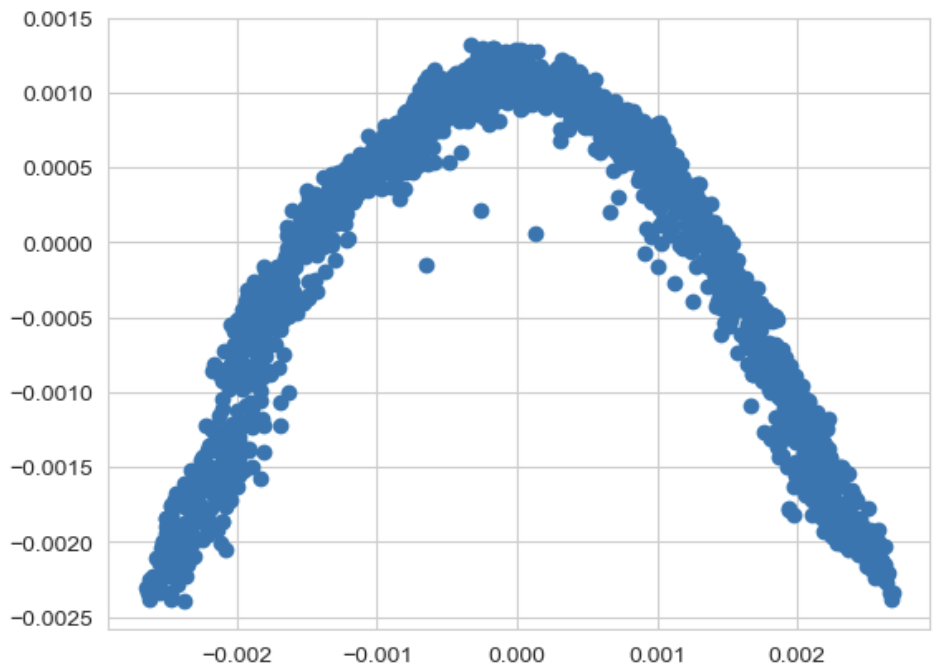
\includegraphics[width=\linewidth]{figures/diffmap_1d_plot.png}
      \caption{$d=1$}
      \label{fig:sub1}
    \end{subfigure}
    \hfill
    \begin{subfigure}{0.49\textwidth}
      \centering
      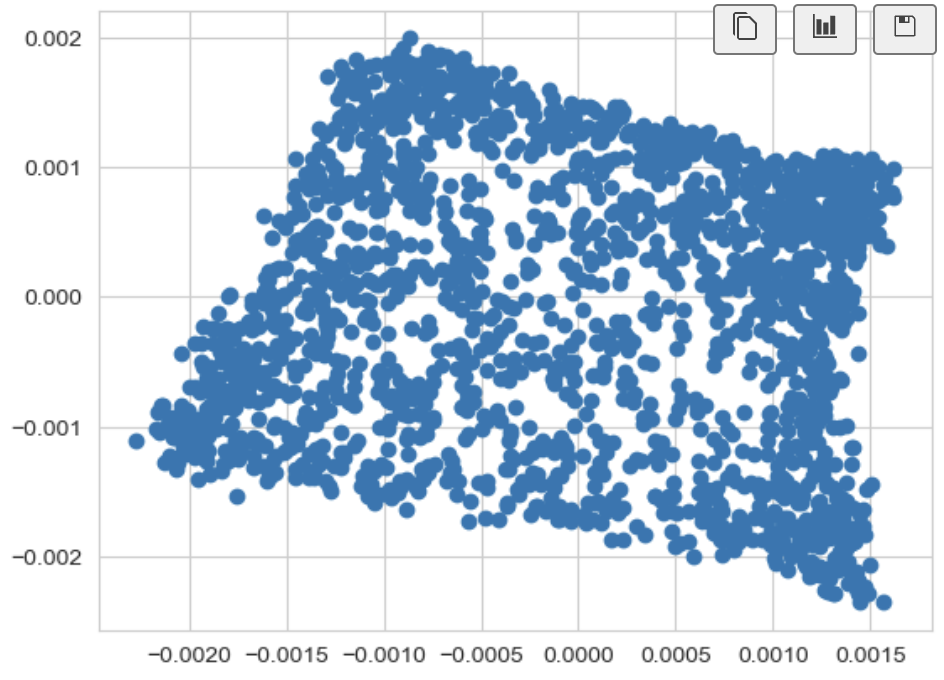
\includegraphics[width=\linewidth]{figures/diffmap_2d_plot.png}
      \caption{$d=2$}
      \label{fig:cube_diffmap_plots_d2}
    \end{subfigure}

  
    \caption{Diffusion map scatter plot of the first two extracted coordinates from 1d and 2d GIRGs.}
    \label{fig:cube_diffmap_plots_d1and2}
\end{figure}


\begin{figure}
    \centering

    \begin{subfigure}{0.49\textwidth}
      \centering
      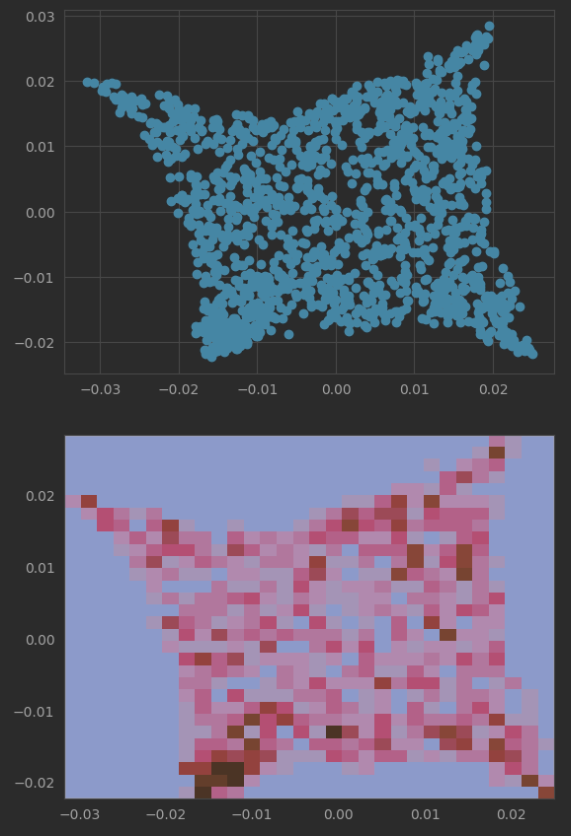
\includegraphics[width=\linewidth]{figures/diffmap_plot_nonuniformed.png}
      \caption{2d GIRG non-uniformed}
      \label{fig:sub1}
    \end{subfigure}
    \hfill
    \begin{subfigure}{0.49\textwidth}
      \centering
      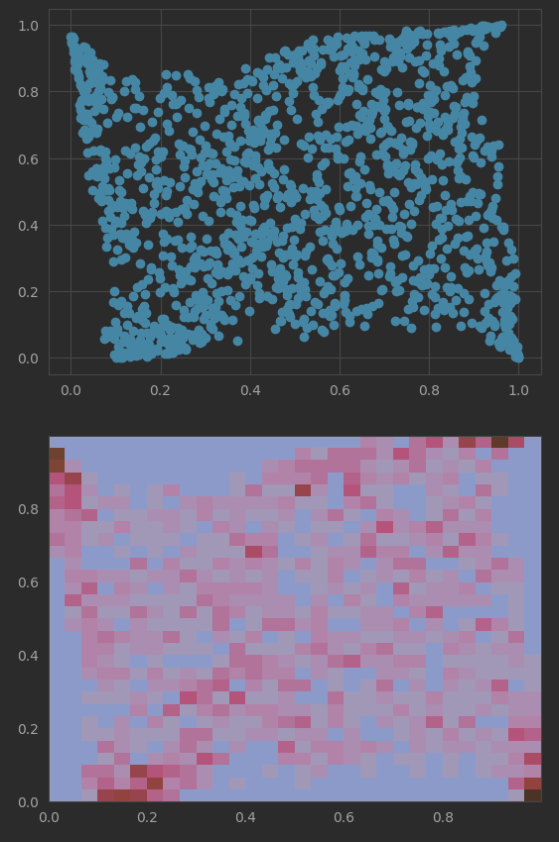
\includegraphics[width=\linewidth]{figures/diffmap_plot_uniformed.png}
      \caption{2d GIRG uniformed}
      \label{fig:sub2}
    \end{subfigure}
  
    \vspace{1em}
  
    \begin{subfigure}{0.49\textwidth}
      \centering
      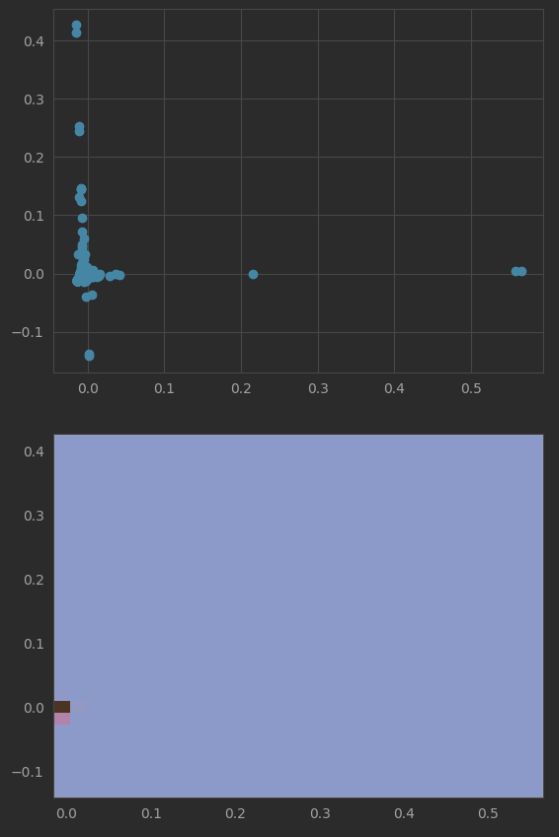
\includegraphics[width=\linewidth]{figures/real_diffmap_plot_nonuniformed.png}
      \caption{socfb-Amherst41 non-uniformed}
      \label{fig:sub3}
    \end{subfigure}
    \hfill
    \begin{subfigure}{0.49\textwidth}
      \centering
      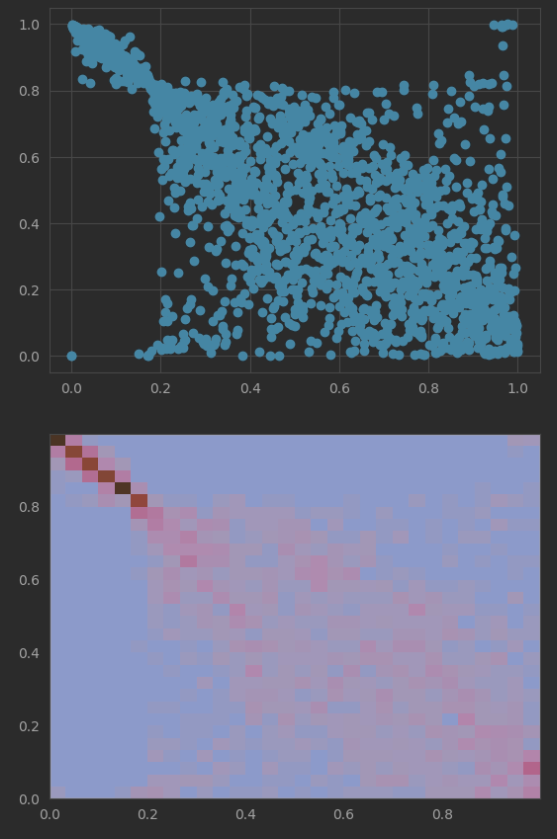
\includegraphics[width=\linewidth]{figures/real_diffmap_plot_uniformed.png}
      \caption{socfb-Amherst41 uniformed}
      \label{fig:sub4}
    \end{subfigure}
  
    \caption{Diffusion map scatter plot of the first two extracted coordinates, with and without using an additional uniform square remapping}
    \label{fig:diffmap_uniformed_vs_nonuniformed}
\end{figure}


\begin{figure}
  \centering

  \begin{subfigure}{0.9\textwidth}
    \centering
    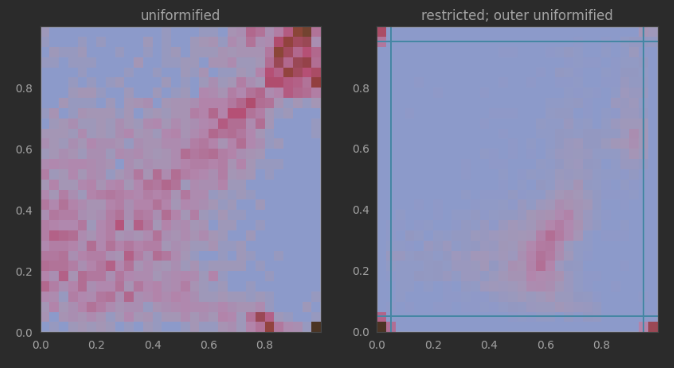
\includegraphics[width=\linewidth]{figures/Rice31_2d_diffmaps}
    \caption{Rice31}
    \label{fig:sub1}
  \end{subfigure}

  \vspace{1em}
  
  \begin{subfigure}{0.9\textwidth}
    \centering
    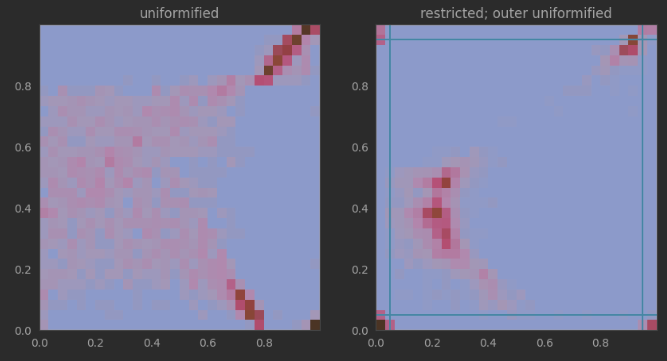
\includegraphics[width=\linewidth]{figures/Bowdoin47_2d_diffmaps}
    \caption{Bowdoin47}
    \label{fig:sub2}
  \end{subfigure}

  \vspace{1em}

  \begin{subfigure}{0.9\textwidth}
    \centering
    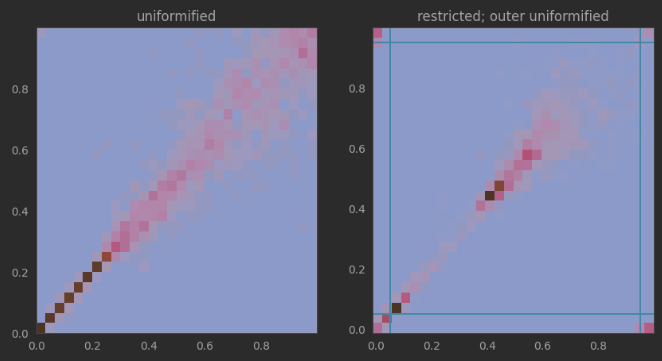
\includegraphics[width=\linewidth]{figures/Simmons81_2d_diffmaps.png}
    \caption{Simmons81}
    \label{fig:sub3}
  \end{subfigure}


  \caption{two methods for rescaling/shifting diffusion maps into the cube - done here for d=2 truncations. The blue lines for the restricted version show the border at which points are outer uniformified.}
  \label{fig:uniformifed_vs_restricted_rescaling}
\end{figure}



\paragraph{Toroidal GIRGs} Interestingly Toroidal GIRGs are differentiated from Cube GIRGs in that the diffusion map requires $2d$ coordinates to capture the Torus geometry instead of just $d$ for the cube. The natural diffusion map of a 1D Torus GIRG ends up being a 2D circle about the origin; 2 larger eigenvalues $\lambda_2, \lambda_3$ are necessary. 


A final issue with diffusion maps is that points seem to end up concentrated in corners/edges. My hypothesis is that this is because e.g. on a 1D line segment, it's hard to distinguish somewhat left and very left points - in the end the diffusion cloud bias is still just left leaning. Not sure how much of a problem this is.

\paragraph{Restricted Rescaling} This method works to bias less towards a uniformly distributed prior while still mapping points into a reasonable geometric space.
Empirically, the diffusion map coordinates of the facebook graphs often have $\geq 90\%$ of the nodes concentrated in a small parcel, with only a few nodes having extremely far out locations.
This defeats the simple rescaling method of $x \gets \frac{x - x_{\min}}{x_{\max} - x_{\min}}$ as most nodes will end up very tightly packed. Instead we rescale the central nodes: those whose joint coordinate-wise percentiles lie in $[5\%, 95\%]^d$.
These nodes are linearly scaled to the $[0.05, 0.95]^d$ cube. Finally the outlying nodes are percentile rescaled (non-linearly) to the upper/lower cube margins.
This method is shown in comparison for a few graphs in \cref{fig:uniformifed_vs_restricted_rescaling}


TODO 

- fuller analysis of different diffmap modes: 'uniformify', 'cubify' and 'cuboidify', comparing performance on real life and synthetic graphs

- presentation of the small degree stochastic walk tweak which improves diffusion map performance:
\begin{verbatim}
# Empirically this gamma seems to work well. 
# It discourages taking edges to popular nhbs.
gamma = 0.9
M_tilde = scipy.sparse.diags(1 / D) @ A @ scipy.sparse.diags(D ** (-gamma))
M_tilde = scipy.sparse.diags(np.array(1 / M_tilde.sum(axis=-1)).squeeze()) @ M_tild
\end{verbatim}

- is it true that diffusion map tends to cluster representations edges rather than being more uniform? Empricially seems to happen in 2D but not 1D?

